\documentclass[a4paper,12pt]{article}
\usepackage{fancyhdr}
\usepackage{geometry}
\usepackage{setspace}
\usepackage{graphicx}
\usepackage{amsmath}
\usepackage{amsfonts}
\usepackage{algorithm}
\usepackage{algorithmicx}
\usepackage{wrapfig}
\usepackage{indentfirst}

%To Do: 
%	[] Spruce up Abstract, Spruce up background (what mri is, relaxation times, maybe include graphs of exponentially dependent functions) 
%	[] Reword some of Canny Edge Detection section (use source Ed sent me), maybe include visuals of binning, gradient directions, and such
%	[] Add to design of system (mention synced folders briefly, and directory formats), and concentration
%	[] Add to Synthesis of MnCl
%	[1] Write about Results for Edge Detection
%	[]		Issues: Noise and Such, maybe mention Ed's source
%	[2] Write about Results with most optimal conc
%	[] 		Include a sample of pure agar? See what happens!
%	[3] Conclusion: Results Discussion, Future Applications

\setlength\parindent{24pt}

\doublespacing

\begin{document}
	\begin{center}
	\vspace{0.5cm}
	\huge{Applications of Image-Analysis \& Canny Edge Detection in Manganese-Enhanced Magnetic Resonance Imaging}\\
	\vspace{0.5cm}

	\singlespacing
	\small{Patrick C. Stocklin}\\

	\small{Advisor: Edward Van Keuren}

	\small{Georgetown University}\\

	\small{4/24/16}\\
	\end{center}

\begin{section}{Abstract}
\singlespacing

Magnetic Resonance Imaging is an imaging technique used to create images from differing magnetization-vector relaxation times in tissues. By applying a constant magnetic field, the hydrogen protons' magnetizations are excited and precess about their axes. When hit by a radio frequency pulse, they are excited but return to their low energy states and emit energy. MRI contrast agents alter the differences in these relaxation times by introducing minute heterogenous magnetic fields. This paper discusses the possible applications of image-analysis techniques such as Canny edge detection towards observing the effectiveness of contrast agents in MRIs. The fall semester was designated as a period to investigate feature-extraction and other various techniques in image-analysis. Professor Van Keuren and I both focused our attention on Canny edge detection, in hopes that it would yield promising applications in our research. The spring semester was more focused on the applications of image-analysis on manganese chloride contrast agents. Multiple samples of manganese chloride with varying concentrations were synthesized and imaged in hopes of finding a promising contrast agent for $T_1$ and $T_2$ imaging. I also spent the spring semester constructing a stand-alone linux-based system for streamlining the analysis of sample images, as well as creating methods for determining the most effective concentration for a manganese-based contrast agent.

%Add about what was found

\end{section}

\newpage
\doublespacing
%%%Things to Add for Sources:
%%%Pictures of Different Thresholds
%%%1D case for gradients.http://suraj.lums.edu.pk/~cs436a02/CannyImplementation.htm
%%%Modeling Intensity Changes (step edge, sharp edge, roof edge, ridge edge)
%%%Roberts, Prewitt, Sobel


\begin{section}{Background Information}

%MRI INFO FROM BRADY/OXFORD SLIDES
%T1-weighted image TR=14ms, TE = 50ms,
%T2-weighted image TR=4000ms, TE = 100ms
%H protons with two spin states are either precessing along or against the external magnetic field
%Bombarded with RF energy, at certain resonant (larmor) freqs the proton flips to high energy states
%Applying pulse at 90 degrees to the B field

%Relaxation T1
%For nuc to return to low energy states the spin system must be exposed to an EM field oscillating with a freq at or close to Larmor freq
%This can occur by the nuc being stimulated by surrounding nuc, occurs in exponential manner
%corresponds to the time req for the system to return to 63 percent of eq when exposed to 90 deg

%Saturation Recovery of Mz back to Mo

%Contribution of all spins is tipped into x,y plane, dephases in the x,y plane

%Relaxation T2, 
%immediately after pulse is applied, spins dephase and signal decreases
%Approximately 10x smaller than T1

%Maybe mention K space and FFT


\subsection{Magnetic Resonance Imaging}
Magnetic Resonance Imaging (MRI) is an imaging techinique used to visualize the anatomy and physiological topology of living organisms. By using powerful externally-applied magnetic fields, scientists and physicians are able to render detailed images of the human body without exposing the patient to potentially lethal forms of radiation. It is this exact reason why magnetic resonance imaging is the predominantly-favored investigative tool for detecting and battling deadly cancer cells. MRI is generally agreed upon to be superior to Computed Tomography (CT) scans for neurobiological visualization because it avoids any harmful exposure to radiation and offers a more detailed image of the grey and white matter in the central nervous system$\cite{1}$.
MRIs also allow for a multitude of images to be taken over a short span of time and may be used to monitor neural or vascular activity as the subject is placed under time-varying conditions or stimulation$\cite{1}\cite{2}$.
Thus it is said to be the leading imaging technique for neuroimaging. \

%Change this section to be about how MRIs work
In the context of this paper, MRI scans of contrast agents will be processed and analyzed to highlight regions of lighter or darker intensity produced by aforementioned contrast agents. Hopefully, by learning more about these contrast agents, we will discover new ways to implement Magnetic Resonance Imaging to effectively diagnose anatomical complications.


\newpage
\subsubsection{MRI Procedure}
Because the human body is mostly comprised of water molecules containing single protons in the nuclei of the Hydrogen atoms, MRI has proven to be an effective means of rendering anatomical images. The hydrogen protons within the area of interest are placed under with a strong, constant magnetic field.
Most clinical MRI machines typically operate between 0.7 - 2.0 Teslas$\cite{3}$. 
The protons' magnetic moment is temporarly altered, precessing about the direction of the applied magnetic-field $\cite{2}$. 
A radio frequency pulse is then simultaneously applied to the patient, causing the protons to become excited out of a state of equilibrium.
This precession then yields a momentary change in the magnetic flux through the hydrogen atom, which then creates a signal that the MRI scanner interprets. The collection of signals are then processed according to their respective frequencies emitted, and the final produced image is obtained by applying a 2-D Fourier transformation across the spatial-frequency domain. 
The signal frequency is directly proportional to the period of time it takes for the protons to return to their low-energy equiilibrium state. This is known as the relaxation period $\cite{3}$. 
More specifically, the recovery of the longitudinal component of the proton's magnetization is classified as $T_1$ relaxation. This is essentially associated with the number of Hydrogen nuclei with parallel spin versus the number of nuclei with anti-parallel spin $\cite{3}$. 
The loss of phase coherence in the proton's transversal plane is responsible for the transversal relaxation, known as $T_2$ relaxation. This relaxation time is associated with the number of hydrogen nuclei in phase with each other $\cite{3}$. 
Both $T_1$ and $T_2$ relaxation rates govern the time it takes for the protons to return to equilibrium.


\newpage
\subsubsection{$T_1$ Relaxation}
$T_1$, or {\em Spin-Lattice Relaxation Time}, is the time required for the magnetization vector to recover 63 percent ($[1-(\frac{1}{e})]$) of its longitudinal magnetization. It characterizes the exponential rate at which the longitudinal component of magnetization reaches equilibrium $\cite{3}$. This value is dependent on the hydrogen proton's environment, and can be altered by the presence of ferromagnetic or paramagnetic particles $\cite{3}$. The longitudinal component of magnetization may be defined by the following time-dependent equation:

\begin{center}
$M_Z(t) = M_{Z,Eq}(1 - e^{-\frac{t}{T_1}})$ 
\end{center}

%Ed says I may have to include more information for this section
An MRI image may be $T_1$ weighted by adjusting the {\em Echo Time}, $T_E$, and {\em Repitition Time}, $T_R$, such that the values obey a conventional spin-echo sequence $\cite{4}$. The {\em Echo Time} may be thought of as the time period following excitation which the proton's signal is read $\cite{4}$. The {\em Repitition Time} may be described as the amount of time that exists between successive pulses of signal. The two times may be adjusted to heavily favor a $T_1$ signal and reduce the amount of contribution by the $T_2$ signal $\cite{4}$. By setting these short $T_R$ and $T_E$ times (typically on the order of $< 750$ ms and $< 40$ ms, respectively), the image will heavily favor image contrast caused by the longitudinal component of magnetization $\cite{4}$.

\subsubsection{$T_2$ Relaxation}
$T_2$, or {\em Spin-Spin Relaxation Time}, is the time required for the transverse component of magnetization to return 37 percent ($\frac{1}{e}$) of its initial magnetization. $T_2$ relaxation typically occurs more quickly than that of Spin-Lattice Relaxation Times $\cite{4}$. Like $T_1$, $T_2$ is dependent on the proton's environment. The transversal component of magnetization may be defined by the following equation:

\begin{center}
$M_{XY}(t) = M_{XY}(0)e^{-\frac{t}{T_2}}$ 
\end{center}

%Ed says "Also Point Out that T1 and T2 are characterized by measuring different magnetization directions (not just changing echo times)"

$T_2$ weighted images may be derived by selecting a $T_E$ that is on the order of the contrast agents {\em Spin-Spin Relaxation Time}. This reduces the information gained by $T_1$ because we are now allowing the excited protons' spins to return to equilibrium before excitation $\cite{4}$.

\subsubsection{Contrast Agents}

The varying brightness contrast in the resulting images is created by the difference in the strength of the nuclear magnetic resonance signal recovered from the detectors. 
%Different types of tissues -> different T1 T2 naturally occuring contrast
This typically is dependent on the difference between the two relaxation times of the nuclei within the sample. Because of the difference between the longitudinal and transverse relaxation times, doctors observe an enhanced or decreased brightness of the sample due to the proton's local environment. In MRI scans, $T_1$ relaxation weighting will characteristically render white matter as white pixels$\cite{3}$. Gray matter within the examined region will appear gray$\cite{3}$. All cerebrospinal fluid, the clear colorless fluid that protects the brain matter, will appear black$\cite{3}$. However, sometimes the contrasting brightness between the types of brain matter will not be as profound or apparent. Therefore, scientists will typically employ the use of a contrast agent to induce a much brighter or darker signal. Because the process from which the MRI images are produce largely depends on the magnetic properties and field around the water molecules, contrast agents are chosen for their magnetic properties$\cite{4}$. 

For the majority of this paper, we will be concerning ourselves with manganese chloride as our contrast agent of interest. Despite being in its infancy as an effective contrast agent, manganese-based paramagnetic particles have been proven to enchance the $T_1$ signal of MRI scans $\cite{5}$. Manganese ions ($Mn^{2+}$) are popular contrast agents in the use of MEMRI (Manganese Enhanced Magnetic Resonance Imaging) $\cite{5}$. It had even been discovered that natural products with a high concentration of manganese can be used for increasing $T_1$ signal $\cite{6}$.

\subsection{Previous Work Done}
Previous work done by Professor Edward Van Keuren in collaboration with the Georgetown University chemistry and physics departments, and the Georgetown Lombardi Comprehensive Cancer Center has made great progress in the exploration for biocompatible nanomaterials as useful contrast agents for MRI scans. Professor Van Keuren's research team has explored the synthesis of copolymers based on the metal-oxo cluster $Mn_8 Fe_8 O_{12}(L)_{16}-(H_2 O)_4$, where L is an acetate or vinyl benzoic acid, coupled with styrene\cite[p.~9040]{7}. The cluster's relaxivity was examined using NMR and confirmed $Mn_8 Fe_8 O_{12}(L)_{16}-(H_2 O)_4$ to be a promising $T_2$ contrast agent. The cluster was also determined to have low cytotoxicity when studied on human prostate cancer cells, potentially allowing it to be used {\em in vivo} for MRI scans\cite[p.~9040]{7}. Testing had also been done on the paramagnetic nanobeads produced by the metal-oxo cluster $Mn_8 Fe_4 - (VBA)_{16}$ copolymerized with styrene. The nanobeads had been confirmed as a potentially useful $T_1$ contrast agent, as their effect on the relaxivity within a polymer matrix only altered the transverse relaxation time ($T_2$) and hardly affected the longitudinal relaxation time ($T_1$)\cite{7}.

More recently, there has been on-going research between the Lombardi Comprehensive Cancer Center and Georgetown University to determine the effect of particle shape and size on $T_2$ Relaxation in contrast agents. Iron oxide nanoparticles had recently been discovered as successful $T_2$ contrast agents.because of the inhomogeneous magnetic field neighboring the ferromagnetic particles $\cite{8}$. Previous research had proven that up to a critical point, the particle size directly alters the $T_2$ of ferromagnetic particles $\cite{8}$. This specific research explored three different particle contrast agents: 1) spherical magnetite ($Fe_3 O_3)$, 2) prolate magnetite, and 3) oblate barium ferrite ($BaFe_{12}O_{19}$). All particles were modeled as spheroidal, and samples consisted of varying concentration levels of contrast agents suspened in layers of 3 percent agar. It was confirmed that the size of the contrast agent did influence the relaxation time up to a limit, but it was observed that the oblate-shaped barium ferrite agent had possessed a relaxivity that surpassed the theoretical limit plotted against surface area per volume $\cite{8}$. Thus the oblate $BaFe_{12}O_{19}$ could prove useful as an effective $T_2$ contrast agent $\cite{8}$.

%\begin{wrapfigure}{R}{0.3\textwidth}
%\begin{center}
%\centering
%\includegraphics[width=0.425\textwidth]{imageregistration.png}
%\caption{registering an image}
%\end{center}
%\end{wrapfigure}

\subsection{Canny Edge Detection}

Because we are interested in highlighting the regions of an MRI image where a contrast agent may brighten or darken the signal, it is necessary to discuss the process of Canny edge detection. Discovered by Australian computer scientist John F. Canny in 1986, Canny Edge Detection is a multi-stage algorithm used to detect a wide range of edges in any given image$\cite{9}$.
This particular edge detection approach attempts to both minimize the low error rate at which it finds edges (find as many as possible) and suppress as much background noise as possible, so as to not produce spurious edges. Canny edge detection is used in many domains of imaging analysis, as it allows for massive amounts of data reduction by extracting only the useful and necessary bits of information. Among all edge detection methods, Canny's implementation is by far the most popular and reliable algorithm to date because it satisfies the three criteria for edge detection by means of calculus of variations$\cite{10}$:\\

\singlespacing
\begin{enumerate}
\item Low error rate for detection edges, the algorithm should detect as many edges as possible  $\cite{11}$.
\item The edge points extracted from the solution must be localized to the center of the edge  $\cite{11}$.
\item Any given edge must only be marked once and image noise must not create spurious false images  $\cite{11}$.
\end{enumerate}
\doublespacing

To achieve this, Canny edge detection requires several steps: 1) Smooth the image in order to reduce noise by applying an arbitrarily sized Gaussian filter across the intensity pixels, 2) Calculate the gradient of the intensity pixels, 3) Reduce the possibility of creating false edges by applying a non-maximum supression to the image, 4) Determine the potential edges by applying a "double threshold", and remove all other weak edges that are not connected to strong ones (Hysteresis). We will now discuss the required steps in greater detail$\cite{12}$.

\subsubsection{Applying the Gaussian filter}

Due to the inherently chaotic and imperfect nature of the process of MRI scans, Canny edge detection would be very susceptible to false positives (detecting unnecessary or weak edges due to unsupressed background noise). Therefore it is essential that we minimize the potential for this unintended detection by smoothing the intensity matrix of our image by masking each pixel with a Gaussian filter$\cite{13}$.%%%%%%%%%
By masking each pixel of our image's intensity matrix, we effectively smooth the image matrix and reduce the amount of chaotic noise that may alter our edge detection's results. For a Gaussian filter with kernel size $(2k+1)\times(2k+1)$: our filter mask may be defined as$\cite{13}$:\\%%%%%%%%%%%%%
\begin{center}
$H_{ij} = \frac{1}{2\pi\sigma^{2}}^{-\frac{(i-k-1)^2+(j-k-1)^2}{2\sigma^2}}$
\end{center}

It is left to the analyst to determine the size of the Gaussian mask.
However it is important to note that as you increase the size of the Gaussian filter, the detector's sensitivity to background noise falls off.
For the sake of a visual example, below is included the Gaussian filter for $\sigma = 1.4$ and of size $5\times5$:\\

\singlespacing
\begin{center}
$A_{GF} = \frac{1}{159}\begin{bmatrix}
	2	&	4	&	5	&	4	&	2\\
	4	&	9	&	{12}	&	9	&	4\\
	5	&	{12}	&	{15}	&	{12}	&	5\\
	4       &       9       &       {12}    &       9       &       4\\
	2       &       4       &       5       &       4       &       2
\end{bmatrix}$
\end{center}
\doublespacing

\subsubsection{Finding the Intensity Gradients}

After smoothing our image to reduce background noise, the next step of Canny edge detection is to calculate the intensity gradients of all image pixels. Given an image matrix of intensity pixels, edges within the image are most likely to be found when there is a strong, well-defined gradient along a uniform direction, since this distinguishes what is a real-world edge. In order to achieve this, a 2-D gradient operator is selected to determine the intensity gradient of each pixel. There are several operators available to calculate the gradients, but the most popular is the $Sobel$ $operator$$\cite{14}$.%%%%%%%%%%%%%%
The 2-Dimensional Sobel operator $|G|$ is a pair of $n\times n$ convolution masks which estimate the gradient in the x and y directions. The Sobel Operator allows us to find the edge strength (gradient) according to $|G|$ = $|G_x|$ + $|G_y|$, where $G_x$ and $G_y$ for mask size 3 are shown below:

\singlespacing
\begin{center}
\[G_x = 
\begin{bmatrix}
-1 & 0 & 1\\
-2 & 0 & 2\\
-1 & 0 & 1\\
\end{bmatrix}
, G_y =
\begin{bmatrix}
-1 & -2 & -1\\
0 & 0 & 0\\
1 & 2 & 1\\
\end{bmatrix}
\]
\end{center}
\doublespacing

Now that we are given the horizontal and vertical gradients of our intensity pixels, calculating the edge gradient is fairly simple.
The edge gradient may trivially be calculated as $\textbf{G} = \sqrt{(G_x)^2 + (G_y)^2}$. 
The direction of the image gradient may be calculated using $atan2$, a trigonometric arctan function which takes in two function parameters and returns an angle from $(-\pi,\pi]$.
However, $atan2$ can be mapped to a range of $[0,2\pi)$ by adding a factor of $2\pi$ to all negative results.
In terms of the typical arctan function, $atan2(y,x)$, for $G_y$ and $G_x$ may be defined as below:

\singlespacing
\begin{center}
\[
atan2(G_y, G_x) = \left\{\def\arraystretch{1.2}%
  \begin{array}{@{}c@{\quad}l@{}}
	arctan(\frac{G_y}{G_x}) & \text{if $G_x$ $>$ 0,}\\
	arctan(\frac{G_y}{G_x}) + \pi & \text{if $G_x$ $<$ 0 and $G_y$ $\geq$ 0,}\\  
	arctan(\frac{G_y}{G_x}) - \pi & \text{if $G_x$ $<$ 0 and $G_y$ $<$ 0,}\\
	+\frac{\pi}{2} & \text{if $G_x$ = 0 and $G_y$ $>$ 0,}\\
	-\frac{\pi}{2} & \text{if $G_x$ = 0 and $G_y$ $<$ 0,}\\
	\text{undefined} & \text{if $G_x$ and $G_y$ = 0}\\
  \end{array}\right.
\]
\end{center}
\doublespacing

Once we have calculated the direction of all pixel intensity gradients, we decide to bin all values into four general directions that may define any edge's direction.
We do this because at the pixel level, all possible lines bisecting a pixel may be oriented exactly four ways.
Given a portion of an $n\times n$ image matrix of intensity pixels:

\singlespacing
\begin{center}
\[
\begin{bmatrix}
x & x & x & x & x\\
x & x & x & x & x\\
x & x & a & x & x\\
x & x & x & x & x\\
x & x & x & x & x\\	
\end{bmatrix}
\]
\end{center}
\doublespacing

we can see that for pixel a, the matrix-scale representation of a possible edge may only be described as a horizontal line, vertical line, or two diagonal lines.
Therefore, we must bin our results from the two-parameter $atan2$ function to describe the direction of a potential edge.
The direction of the edge is always described as being perpendicular to the edge, for example, a nearly vertical edge would be given a direction approximately horizontal.
The four directions we bin our gradient directions are $0^o$ (our horizontal), $45^o$, $90^o$ (vertical), and $135^o$.
The binning function $f(\theta)$ for which we map our directions to our range is defined as:

\singlespacing
\begin{center}
\[
f(\theta) = \left\{\def\arraystretch{1.2}%
  \begin{array}{@{}c@{\quad}l@{}}
	0^o & \text{for $\theta$ in [0,22.5) $\cup$ [157.5,202.5] $\cup$ (337.5,360]}\\
	45^o & \text{for $\theta$ in [22.5,67.5) $\cup$ (202.5,247.5]}\\
	90^o & \text{for $\theta$ in [67.5,112.5) $\cup$ (247.5,292.5]}\\
	135^o & \text{for $\theta$ in [112.5,157.5) $\cup$ (292.5,337.5]}\\
  \end{array}\right.
\]
\end{center} 
\doublespacing

We have now successfully assigned realistic edge-directions for all image pixels corresponding to their intensity gradients.

\subsubsection{Applying non-maximum supression}

What distinguishes Canny's implementation from other edge-detection algorithms is the careful use of edge-thinning$\cite{13}$.%%%%%%%%%
The end result of this edge-thinning step is that all edges should be transformed into edges of pixels with unit width.
The advantages of this process are that the edges are now sharp, precise, and better define the objects or regions we are interested in extracting or analyzing.
Because the edges extracted from the gradient values may still be quite blurred and distorted, we would like to minimize the amount of extraneous edges extracted by removing the weakly defined edges.
This is done by iterating through all of the pixels in our image, and comparing their gradient magnitudes to their neighboring pixels based on their direction. 
A simple explanation of the edge-thinning process is included on the next page in the form of pseudocode:

\newpage
\singlespacing
\begin{algorithm}
\caption{Edge-Thinning $O(n^2)$ run time complexity for $n$x$n$ Matrix}
\begin{tabbing}
1. $\textbf{def}$ \= $thinEdges$(gradImage I): $\hspace{1.5cm}$ $>$Our image-matrix of pixels\\
2. \> for \= $\textbf{pixel}$ in gradImage I:\\
3. \> \> if \= $\textbf{pixel.GradTheta}$ == $0^o$: \\
4. \> \> \> if \= $\textbf{pixel.GradMag}$ \= $< \textbf{EastNeighbor.GradMag}$\\
   \> \> \> \> \> or $<\textbf{WestNeighbor.GradMag}$:\\
5. \> \> \> \> $\textbf{pixel.GradMag}$ = 0 \\
6. \> \> elif $\textbf{pixel.GradTheta}$ == $45^o$: \\
   \> \> \> if $\textbf{pixel.GradMag}$ $< \textbf{NENeighbor.GradMag}$\\
7. \> \> \> \> \> or $<\textbf{SWNeighbor.GradMag}$:\\
8. \> \> \> \> $\textbf{pixel.GradMag}$ = 0 \\
9 .\> \> elif $\textbf{pixel.GradTheta}$ == $90^o$: \\
10 \> \> \> if $\textbf{pixel.GradMag}$ $< \textbf{NorthNeighbor.GradMag}$\\
   \> \> \> \> \> or $<\textbf{SouthNeighbor.GradMag}$:\\
11.\> \> \> \> $\textbf{pixel.GradMage}$ = 0 \\
12.\> \> elif $\textbf{pixel.GradTheta}$ == $135^o$:\\
13.\> \> \> if $\textbf{pixel.GradMag}$ $< \textbf{NWNeighbor.GradMag}$\\
   \> \> \> \> \> or $<\textbf{SENeighbor.GradMag}$:\\
14.\> \> \> \> $\textbf{pixel.GradMag}$ = 0 \\
\end{tabbing}
\end{algorithm}
\doublespacing

As we iterate through all pixel values, each containing a gradient direction and magnitude, we examine the neighboring pixels and decide whether or not we suppress the potential-edge.
A useful way to conceptualize the intended effect of this algorithm is by imagining we are examining a true horizontal edge with a completely verticle gradient direction.
Because we want to thin the potential edges of our region of interest, we should inspect the intensities of the pixels above and below the pixel.
If the pixel gradient's magnitude is the local maximum, we should keep it. 
If there are pixels in the positive or negative direction of the pixel's gradient, then we supress the pixel's weight by assigning its gradient magnitude a value zero.

\subsubsection{Applying double threshold: hysteresis}

After edge-thinning, we finally have a transformed image of precise, small edge-pixels that hopefully accurately describe the objects or regions.
We now wish to finalize our image by classifying the matrix of potential edge-pixels by constructing two gradient magnitude thresholds, $T_h$ and $T_l$ such that $T_h$$>$$T_l$$>$$0$, which will be used to determine whether the pixel is a strong edge or weak edge$\cite{15}$.%%%%%%%%%%%%%%%
Again, we iterate through our image matrix comparing the pixel's gradient magnitude to our two chosen thresholds.
If the pixel's magnitude is greater than both thresholds, we may classify it as a strong pixel.
If the pixel's magnitude is smaller than both thresholds, the pixel may be supressed or disregarded completely.
However, if the pixel's magnitude is less than the upper threshold, but greater than the smaller threshold, then we classify it as a weak pixel.
Weak pixels may or may not be part of the true edge of our object, this is determined by its connectedness to a strong pixel in its neighborhood.\\

The process of hysteresis is a recursive approach for mapping edges based on pixel-connectedness. As we traverse the image matrix, the first strong pixel encountered with a magnitude greater than our upper threshold is declared an edge$\cite{15}$.%%%%% 
From the edge pixel, we examine its 8 adjacent neighbor-pixels: if any neighboring pixels are also defined to be strong pixels, they are appended to the edge object that maps our edge.
Those pixels are further examined for adjacent strong pixels until we encounter our base case of there being only adjacent weak pixels.
A data structure such as a map must be used to prevent the revisitation of previously encountered pixels $\cite{15}$.

Now we must handle whether or not we preserve the weak pixels.
The process is similar to mapping the strong pixels to edges in that we examine every weak pixel's 8 surrounding neighbor-pixels. 
If there are any strong edge pixels connected to the pixel in question, then we decide that it is a pixel associated with an edge and not just background noise.\\

\begin{center}
\includegraphics[scale=0.3]{einstein_original.png}
\includegraphics[scale=0.3]{einstein_100_200.png}

Original Image \hspace{25mm} $T_h$ = 200, $T_l$ = 100
\end{center}
\begin{center}
\includegraphics[scale=0.3]{einstein_100_300.png}
\includegraphics[scale=0.3]{einstein_150_200.png}

$T_h$ = 300, $T_l$ = 100 \hspace{20mm} $T_h$ = 200, $T_l$ = 150
\end{center}

Due to the fact that it is left to the analyst to determine the limiting gradient values, it is worth noting the effects of altering the threshold values $T_h$ and $T_l$.
As one increases the upper-threshold $T_h$, fewer pixels will satisfy the criteria for being a strong edge, so there will be fewer edges produced in the final image $\cite{16}$.
However, as you increase the lower-threshold $T_l$, fewer pixels will satisfy the condition for being a weak edge, so the edges that are rendered will possess lengths that are much smaller $\cite{17}$.
The degree to which we alter the threshold values depends on the context and desired output of our edge detection, and thus will need to be fine-tuned. 

We can briefly verify the consequences of altering the thresholds by observing the four images of Einstein above. The original image is then processed through Canny edge detection with gradient threshold values of 100 for lower bound, 200 for upper bound. By raising the upper bound to 300, we reduce the number of strong pixels that fall below a gradient value of less than 300, so there are now fewer edge objects being rendered. By raising the lower bound to 150, we reduce the length of the resulting edges because we now have a higher metric for filtering the weak pixels that are adjacent to strong ones. Both increases to the thresholds yield a fewer amount of edges, but the reasons for the decrease in pixelated edges are different.

\subsection{Image Registration}

One of the nuances of biomedical imaging analysis is having to establish a universal coordinate basis for any two images we wish to analyze and compare. In an ideal scenario, all images taken of a patient would be oriented in such a way that, if one were to stack the images on top of each other, the body and organs would be perfectly aligned. However, this is obviously not the case: as the scanner produces multiple images, the patient may slightly move or turn, creating an image with features that are uncentered or rotated. This makes comparing two rendered images incredibly difficult, so it is imperative that both images are transformed so that their relevent features are aligned in the same coordinate system. 

\newpage
\subsection{Technologies and Frameworks}

This section will briefly cover the related technologies used in constructing and designing the image-processing system I have created.

\singlespacing

\subsubsection{VirtualBox}


\begin{wrapfigure}{L}{0.5\textwidth}
\centering
\includegraphics[width=0.15\textwidth]{Virtualbox_logo.png}
\caption{VirtualBox}
\end{wrapfigure}

VirtualBox is an open-source memory-hosted (as opposed to hardware-hosted) hypervisor developed by Innotek GmbH in 2007 and acquired by Oracle Corporation in 2010 $\cite{18}$. 
It is cross-platform compatible as long as the machine adheres to an x86 CPU architecture $\cite{18}$. VirtualBox allows the user to support and manage their own virtual machines running on their host computer. Virtualization is a useful technique because it offers an easy and streamlined solution to shipping software packages and systems. Virtualization also offers the user the ability to spin up multiple operating systems and a more stable and isolated environment for testing and stressing of software and systems. To this day, Vagrant continues to grow and garner community support through the Open Source Project $\cite{18}$.

\begin{wrapfigure}{R}{0.2\textwidth}
\begin{center}
\includegraphics[width=0.15\textwidth]{Vagrant.png}
\end{center}
\end{wrapfigure}

\subsubsection{Vagrant}

Vagrant is another open-source software written in Ruby and used for configuring virtual environments $\cite{19}$.. It was developed and released by HashiCorp in 2010 and continues to grow. Vagrant is commonly used as a wrapper in conjunction with virtualization software such as VirtualBox or VMWare. It aims to solve the issue of software refusing to cooperate with a user's unique system or machine for whatever reason. Basically, if it works on one person's machine, it should work on anybody else's so long as they have Vagrant installed. Some of the benefits of using Vagrant include a streamlined, automated provisioning as well as effortless portability $\cite{19}$. 

\subsubsection{Conda}

Conda is an open-source package and environment management system developed by Continuum Analytics and released in 2014 $\cite{20}$. Although it is written primarily in and for Python, it can support packages designed for multiple languages in mind, such as R or C++. It allows the user to seamlessly install package binaries from well-maintained repositories as well as interchangeably switch between versions of software for dependency-integrity. 

\subsubsection{OpenCV}

\begin{wrapfigure}{L}{0.2\textwidth}
\begin{center}
\centering
\includegraphics[width=0.15\textwidth]{OpenCV.png}
%\caption{OpenCV}
\end{center}
\end{wrapfigure}


OpenCV (Open Source Computer Vision) is a cross-platform ensemble of computer-vision functions originally developed by Intel in 1999 in Nizhny Novgorod, Russia $\cite{21}$. It is entirely written in C/C++ and has interfaces for C, C++, Python, Java and MATLAB $\cite{21}$. The project was created as an initiative to further progress computationally intensive processes (such as ray-tracing) by offering a portable, free library of optimized functions that adhered to a well-defined infrastructure which developers could collaborate on. The library offers many vision-applications and statistical learning models such as feature extraction, motion-tracking, classification and learning-trees $\cite{21}$. There was a second release of OpenCV in 2008. Since 2012, the project has been maintained by a non-profit foundation OpenCV.org. 

OpenCV is widely used throughout the globe for a variety of applications. Thanks to its efficient real-time processing power, OpenCV is used for purposes such as detecting swimming pool drownings, intrusions in surveillance video, product quality assurance and rapid, instantaneous facial recognition. It has approximately 2500 optimized computer-vision and machine learning algorithms, with over 9 million downloads worldwide $\cite{21}$.

\subsubsection{ImageJ}

ImageJ is an open-source java-based image-processing software developed by the National Institute of Health $\cite{22}$. It was released in 1997 as a successor to the freeware image analysis software titled NIH Image. It contains an extensible toolset for image manipulation and can accommodate most image formats (.GIF, .JPEG, .PNG, .BMP). By utilizing an in-memory stack of images per window, it can quickly perform such calculations as contrast manipulation, convolution, Fourier analysis, and smoothing/sharpening $\cite{22}$. ImageJ was used for sample-quality inspection after their preparation. Currently, it is one of the fastest java-written image-processing softwares to exist, clocking in at 40 million pixels per second, or an entire 2048x2048 image in 0.1 seconds $\cite{22}$.

\end{section}


\newpage
\begin{section}{Methods}

This section will provide a detailed explanation of the innerworkings of the system I have created to perform edge-detection on the manganese chloride images. There will also be a step-by-step documentation of the preparation and synthesis of the imaged samples.


\subsection{Design of System}

This section will walk through the construction and design of the image-analysis system I have created. I will detail the inner-workings and function of the system.

\subsubsection{Benefits and Utility}

As the reader may have noticed in the subsection detailing the relevant technologies, every single software listed was categorized as open source software. One of the most stifling drawbacks of depending on other image-analysis software (such as MATLAB) is that the software is typically labeled as proprietary, or closed-source software. This poses several issues: 1) researchers and scientists may not have the resources to purchase a legal license to use the software 2) the code which the algorithms are implemented with is not available to the public, and 3) collaborative development is non-existent outside the owner of the license. By including only open source technologies, I have created a completely free and easily-accessible tool for other researchers to perform automated edge-detection on a corpus of images. Thanks to the layer of abstraction and hardware-isolation provided by virtualization software such as Vagrant and VirtualBox, the system is not heaviliy reliant on the user-machine's dependencies. Thus the system is effortless to deploy for whomever would be interested. 

\subsubsection{An Overhead View}

Below is a simple diagram that adequately describes the interactions and encapsulation of all the software my system is composed of.

\begin{center}
\includegraphics[scale=0.35]{SystemDesign.png}
\end{center}

With VirtualBox running, the Vagrant environment can be initialized if it had not been previously instantiated. The virtual machine can be called or killed whenever the user requires its services. If the virtual environment has not been provisioned, the first thing Vagrant will do is pull an Ubuntu 14.04 operating system for our environment to run on. Several bash shell scripts will then be called to configure the system, such as building target/result directories for our image, as well as installing libraries and packages such as Conda and OpenCV. 

After all dependencies have been installed and verified to be working, the user may SSH (secure shell) into the vagrant environment if he/she deems it necessary for any minor tweakings or exploration. Ingesting the images of interest is very simple and requires only a SCP (secure copy) command to safely transfer images from the host machine into the target directory. Once the images of interest have been injected, the user simply executes a python script to analyze all images within the target directory and store the results in a result directory. If the user wishes to do so, he/she may retrieve the resulting images and save them to their host machine with another SCP command.

Anybody can download this system by simply cloning the project's repository from GitHub and following the provided README.md file that walks the user through set-up and use.

\subsection{Synthesis of Manganese Chloride Contrast Agents}

To determine which concentrations of manganese chloride to use for our testing, we first began by taking both $T_1$ and $T_2$ weighted MRI scans of varying concentrations of contrast agent and distilled water in 10mL vials. Concentrations could vary anywhere from 0.01 to 5 parts manganese chloride to water. It was then left to the discretion of the lab-worker to select a range of concentrations that best yielded a brighter image for $T_1$ imaging and a darker image for $T_2$. On the 5th of April, 2016, Xiaowan Zheng and I selected 6 concentrations of 2, 1, 0.5, 0.2, 0.1, and 0.8 as candidate concentrations for the next procedure. All 6 concentrations proved to be hopeful contrast agents in that they produced brighter and darker images for $T_1$ and $T_2$.\\

After selecting our 6 concentrations, we proceeded to recreate the contrast agents in volumes of 20mL. With a 100 $u$Molar solution of manganese chloride we then recreated the concentrations found to be promising by once again mixing with parts of distilled water. The componenents of each contrast agents are below:

\begin{center}
    \begin{tabular}{ | l | l | p{2cm} |}
    \hline
    Concentration & mL of $MnCl_2$ & mL of $H_2O$ \\ \hline
    2 & .4 mL & 19.6 mL  \\ \hline
    1 & .2 mL & 19.8 mL \\ \hline
   .5 & .1 mL & 19.9 mL \\ \hline
   .2 & .05 mL & 19.95 mL \\ \hline
   .1 & .02 mL & 19.98 mL \\ \hline
   .08 & .8 mL of 2uM & 19.2 mL \\ \hline
    \end{tabular}
\end{center}

Once all concentrations have been portioned out, we then set out to mix each contrast agent with heated liquid agar. Because agar solidifies at room temperature, we can stack varying concentrations of contrast agent on top of each other. So we first mix 200 mL of distilled $H_2 O$ with 6 grams of agar to create a solution of 3 percent pure agar. The agar solution is then heated in a microwave until the solution is homogeneous enough that the agar particles are distributed uniformly enough. To remove air bubbles from the agar, we place the solution in a heat bath. Air bubbles could potentially ruin our samples' images, so it was imperative to remove them as best as possible.\\

\begin{center}
\includegraphics[scale=0.5]{6tray.png}
\end{center}

Once our solution of agar was as homogeneous as possible, we then combined 5 mL of each contrast agent with 5 mL of agar. Each mixture was placed into one of 6 wells and left to dry. The photograph above shows mixtures, from right to left, of concentrations 2, 1, 0.5, 0.2, 0.1, 0.08 (empty). Once the wells were hardened, we were finally able to slice cubettes of contrast agent for injecting into our final sample to observe the effectiveness of the contrast agents.

We then began to create our 50 mL vial containing layers of hardened agar mixed with contrast agents of different concentrations. The first layer at the bottom of the vial was filled with pure agar. This first layer provides the ground that the first cubette of manganese chloride will rest upon. To extract the cubette, a precision knife was used to slice the jello-like agent into many sections. Upon inspection, the cubette that was the most uniform in size and substance, meaning no bubbles, tears, or miscellaneous impurities, was selected as the candidate. The first candidate cubette of concentration 2 was placed on the level of pure agar. The space surrounding the candidate cubette was filled with pure agar and left to solidify, providing the next level for the sequential cubette to sit on. It is important to note that the surrounding agar had to provide a buffer between each cubette, so each cubette was completely submerged in surrounding agar. This process was repeated until we had selected candidate cubettes from each concentration. The remainder of the vial was filled with agar, and became ready for imaging. \\

%Include side by side of layer by layer image
\begin{center}
\includegraphics[scale=0.4]{sample.png}
\hspace{25mm}
\includegraphics[scale=0.5]{5layers.jpg} \\
\small{A schematic of the 50 mL vial [8], and a cross-sectional image of a sample}
\end{center}

\end{section}

\newpage
\begin{section}{Results}
%Conc 1: 	T1_21 TE = 8.6984, TR = 940
%Conc 1: 	T2_19 TE = 12, TR = 4200
%Conc 0.1: 	T1_16 TE = 8.6984, TR = 940
%Conc 0.1: 	T2_14 TE = 12, TR = 4200

%Talk about sets of samples, parameters, images (mine and ImageJ's), and why there are lack of results
The samples used to perform edge-detection were synthesized using the aforementioned method on the November 11th, 2015. There were only 4 concentrations of manganese chloride included in the set of weighted images (1, 0.1, 0.04, 0.004). Also included is a control pair of weighted images that displays only a slice of pure agar seen from above. All $T_1$ weighted images were taken with $T_E$ = 8.6984ms, $T_R$ = 940ms. All $T_2$ weighted images were taken with parameters $T_E$ = 12.00ms, $T_R$ = 4200ms. It is important to clarify that this batch of images does not accurately represent the intended effect of the contrast agent. Instead of all concentrations showing a brighter signal with $T_1$ and a darker signal with $T_2$, some sets show no observable contrast difference. It may also be the case that $T_2$ weighted images actually show an increased brightness, while some $T_1$ weighted images show a darker signal. Therefore, we will only use this dataset to deduce the validity of samples via Canny edge-detection. 

Because our only set of actual manganese chloride concentrations has been considered unfit for determining their effectiveness as $T_1$ and $T_2$ contrast agents, representative images were created using the image-editing software GIMP. Several sets of images were created to emulate the agents' intended effects. All images were created using a template to ensure uniform dimensions. Any discrepancies between $T_1$ and $T_2$ images or from one concentration to another would negatively influence the quantitative assessment of whether or not a concentration would be a suitable agent. When creating the collection of artificial images, specific gray-scale quantities were taken to ensure that some concentrations were deemed more suitable than others. The surrounding agar was always created using a grayscale value of 195, with a pixel shade of 210 applied as an airbrush to simulate noise. The airbrush was separately applied to each image to emulate the agar's response to $T_1$ and $T_2$ weighting in order to demonstrate the necessity of normalizing our cubettes' effectiveness. 

For $T_1$ weighting, all cubette regions were filled with shades that were considerably brighter than the surrounding agar. $T_2$ images were filled with shades that were noticeably darker than the surrounding agar. Sets of images were constructed such that each pair varied slightly in contrast-difference. This was done by shading one or both cubette regions with slightly greater or smaller pixel-values. Cubette regions were also edited to emulate noise and agent non-uniformity.

The set of agents created on April 5th, 2016 (concentrations 2, 1, 0.5, 0.2, 0.1, and 0.08) were imaged shortly after their synthesis. Because the produced images did not display any significant changes in brightness, they were ultimately discarded as a failed batch. This set of images will neither be included nor discussed. 

Insert table of Image Properties and Additions at end? Along with set of all images

\subsection{Determining sample "goodness" with edge-detection}

A valid sample will obey the two following clauses: 

\singlespacing
\begin{enumerate}
\item The sample's cubettes are uniform in consistency, with no noticeable impurities
\item The sample's cubettes which are expected to show an enhanced signal do display a change in pixel-brightness
\end{enumerate}
\doublespacing

A sample that fails to meet the above requirements can not be considered unquestionably useful. If the cubette appears non-uniform and afflicted with multiple impurities, then it cannot be determined whether or not the contrast is responsible for the change in brightness. An impurity can be a tear in the gel-cubette, a trapped air-bubble that was caught between the surrounding agar and cubette during insertion, or an unexpected suspended particle that was not intended to be included. The synthesis procedure aims to minimize the possibility for impurities: the agar is distributed as uniformly as possible to ensure no clumps of particles and the air-bubbles are removed with the use of a heat-bath. All impurities that would significantly influence the goodness of a sample are easily detected by Canny edge detection. However the difficulty lies in distinguishing anomalies from background noise. A careful application of edge-detection will determine whether or not a pair of images satisfies both conditions. 

\subsubsection{Determining Optimal Thresholds}
%Finding Optimal Thresholds: Noise, Pure Agar, Thresholds until we get no edges
%First Requirement, Gunky T_2 image with varying thresholds vs nice T_1 image with varything thresholds
%Second Requirement, Nice T_1 brighter image, so include them boys


Images to Include: Edge Detections
	-Lots of Noise (Pure Agar)
	-T2 with lots of gunk in the middle
		-Varying Thresholds
	-T1 with blank cubette in the middle
		-Varying Thresholds

\subsection{Determining the most optimal $Mn-Cl_2$ Concentration}

We are interested in determining the most optimal concentration of contrast agent. "Most optimal" would mean the concentration that would excellently produce brighter images with $T_1$-weighting and darker images with $T_2$-weighting. It has been demonstrated that some concentrations yield resulting images that are either all brighter, all darker, or display no real influence on the image's intensity. This could either have been due the contrast agent's concentration alone, or a poor choice in MRI parameters ({\em Echo-Time, Relaxation-Time, radio pulse frequency, etc.}). A concentration's efficiency for a specific set of parameters could be quantified as the difference in pixel-intensity. Greater differences in the intensity would signify an increased effectiveness for a concentration. The following sections will describe my solution to this problem, as well as its obstacles it encountered.

Talk about the theoretical model of there being critical point of concentration that does not yield effective contrast

\subsubsection{Assumptions \& Method}

In order to approach this problem, some assumptions must be made about our images. Their resolutions will appear following the description of the solution. The assumptions are as follows:

\singlespacing
\begin{enumerate}
\item The sample's cubettes of contrast agent are uniform in dimension
\item The sample's cubettes' locations do not deviate from each other
\item The sample's surrounding agar does not experience intensity-contrast
\end{enumerate}
\doublespacing

The first assumption is critical because it directly influences the metric on which we gauge the concentration's effectiveness. If one concentration's cubette covers more of the image than another concentration's cubette, then we could incorrectly label one concentration as more or less effective than its competitors. The second assumption makes the solution possible, because feature-extraction of this nature would be impossible if images were to be misaligned in their coordinate-planes. The third assumption removes the task of normalizing the result to verify the true efficiency of our concentrations. All assumptions are discussed in further detail later.

The Python file titled {\em findBestConcentration.py} in the {\em scripts} directory contains all the necessary calculations and functions to successfully determine the "most optimal" concentration given a set of $T_1$ and $T_2$ images. First, all images in the target-folder's subdirectories are loaded and paired according to their concentrations. For every pair of $T_1$ and $T_2$ images, the following is done:

\singlespacing
\begin{enumerate}
\item Extract N-horizontal pixel vectors from the center of both images (N is user-defined)
\item Apply a 1-D Gaussian convolution mask to further reduce noise for every pixel vector
\item For every horizontal pixel vector find the absolute value of the difference between its corresponding "sibling" pixel and store as a vector
\item Normalize this pixel-difference vector by removing the pixels produced by the agar's intensity contrast
\item Treat the vector of pixel-differences as a curve and calculate the area underneath the curve
\end{enumerate}

\doublespacing

The concentrations are then sorted according to their results from determining the area under their pixel-difference vector. The concentrations with the largest areas are recommended as an optimal contrast agent.

\subsubsection{Issues and Solutions}

As previously mentioned, the assumptions made to ensure this solution's confidence and precision were 1) the cubettes do not vary in size from one concentration to another, 2) the cubettes do not appear to move from image to image, and 3) the pure agar does not experience notable intensity-change. Their influence on the above approach for determining the best concentration levels will now be discussed, along with possible solutions.

The first assumption was installed to remove the bias some concentrations would create when calculating the area under the curve. For larger cubettes of contrast agent, more area would lie underneath the pixel-difference curve and would thus yield a deceptively larger or smaller area. This augmented area would misrepresent the concentration's effectiveness, so the assumption is made that all cubettes are uniform. One potential approach to overcome this obstacle would be to standardize the region under which we calculate our area/efficiency. An application of 1-Dimensional Canny edge detection would be used to determine the locations along the pixel-difference vectors where intensity-transition is highest. These locations would represent where the pure agar turns into brighter or darker regions containing contrast agents. The boundaries surrounding the smallest regions would then be applied to all concentrations to ensure the areas under the curves would be taken over a uniform range. This would then represent a more realistic efficiency-score for our concentrations.

The second assumption was created to remove the necessity for image-registration. If two cubettes of the same concentration were slightly misaligned, then the calculated efficiency would not be an accurate representation. If it is assumed that the camera and/or sample does not move between $T_1$ and $T_2$ images, then it is no longer necessary to align the images. To resolve this issue, all pairs of images would be registered with respect to each other features and origins.

The third assumption requires the algorithm to account for unexpected brightness-contrast for the surrounding agar. If for one concentration the agar had produced varying intensities, this would leave our concentrations' true efficiencies unnormalized. Because the surrounding agar is not uniform in brightness, this begs the question: How do we know what values to reduce our pixel-difference vector by? One approach may be to discretize and bin pixels outside the region of highest pixel-contrast and then reduce their influence on the cubette's pixel-contrast. This would result in a much more accurate and representative efficiency score for a given concentration. 

\subsubsection{Results}

Because of the lack of sample sets with desirable characteristics (brighter image in $T_1$, darker image in $T_2$), the aforementioned algorithm was preformed on several sets of artificial, but representative sample-images created in GIMP. Some of the images can be seen below:

\begin{center}
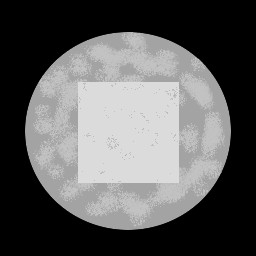
\includegraphics[scale=0.25]{T1.jpg}
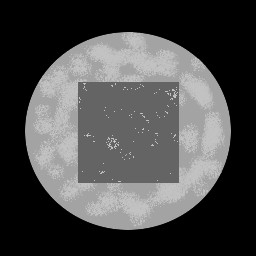
\includegraphics[scale=0.25]{T2.jpg}
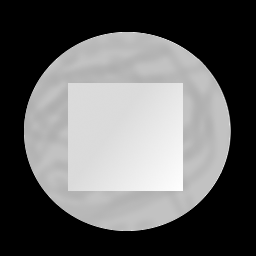
\includegraphics[scale=0.25]{T1*.png}
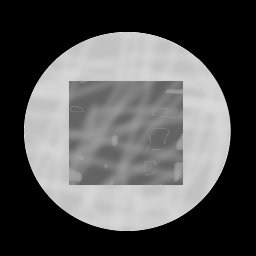
\includegraphics[scale=0.25]{T2*.png}
\end{center}
\begin{center}
\small{Two test sets of $T_1$ and $T_2$ images, (Set No. 2 $T_1$ and $T_2$, Set No. 3 $T_1$ and $T_2$)}
\end{center}

Line graphs representing the pixel-intensities for ideal $T_1$ and $T_2$ images were taken during testing and may be found below:

\begin{center}
\includegraphics[scale=0.35]{SingleSlice_Test3_T1.png}
\includegraphics[scale=0.35]{SingleSlice_Test3_T2.png}
\end{center}

Both slices of pixel-values were taken laterally along the middle of the image and interesect the regions of enhanced and reduced brightness. Both graphs belong to test set 3, as seen above. It is important to note that the surrounding agar does noticeably vary from $T_1$ to $T_2$, and was done so to demonstrate the necessity for normalizing the efficiency.\\

For smoothing the horizontal slices of pixels, a 1-D Gaussian Filter was selected with size 5 and $\sigma = 1.4$:

\begin{center}
$G_F = \frac{1}{159}
\begin{matrix}
[ 5 & 12 & 15 & 12 & 5 ]
\end{matrix}$
\end{center}
	
Once applied, the final pixel-difference vector represented by a line graph appeared like so:

\begin{center}
\includegraphics[scale=0.6]{Unnormalized_GF_Test3.png}
\end{center}

It is easy to see that because we left the vector unnormalized, regions of surrounding pure agar still influence the area underneath the curve. This demonstrates the necessity for determining the contribution to the efficiency-score made by the slight contrast in the agar. It is easy to see how a 1-Dimensional application of Canny edge detection would yield a position-approximation for region boundaries. Because the intensity-gradient changes so dramatically around the region of transition, there would be no difficulty in isolating the region of agar from the cubette.

\end{section}

\newpage
\begin{section}{Conclusion}
\subsection{Results and Discussion}

\subsection{Future Applications}

Talk about collaboration on system
	Turn it into a ML project
	More Image Analysis Techniques

Future Endeavours
\end{section}

\newpage
\singlespacing
\begin{thebibliography}{9}

%Good
\bibitem{1}
Formica D, Silvestri S (April 2004). {\em Biological effects of exposure to magnetic resonance imaging: an overview}. Biomed Eng Online 3: 11. 

%Good
\bibitem{2}
American Society of Neuroradiology, 2013. {\em ACR-ASNR Practice Guideline for the Performance and Interpretation of Magnetic Resonance Imaging (MRI) of the Brian}.

%Good
\bibitem{3}
McRobbie D., et al. MRI, {\em From picture to proton}. 2003

%Good
\bibitem{4}
Malcolm H. Levitt (2001). {\em Spin Dynamics: Basics of Nuclear Magnetic Resonance}. Wiley.

%Good
\bibitem{5}
Koretsky, Alan P.; Silva, Afonso C. (2004). {\em Manganese-enhanced magnetic resonance imaging (MEMRI)}. NMR in Biomedicine 17 (8): 527–31

%Good
\bibitem{6}
Lin, Yi-Jen; Koretsky, Alan P. (1997). {\em Manganese ion enhances T1-weighted MRI during brain activation: An approach to direct imaging of brain function}. Magnetic Resonance in Medicine 38 (3): 378–88.

%Good
\bibitem{7}
Michele Pablico-Langisgan, William Hickling, Emily Japp, Olga Rodriguez, Anup Ghosh, Chris Albanese, Maki Nishida, Edward Van Keuren, Stanley Fricke, Norman Dollahon, Sarah Stoll. 2013, Magnetic Nanobeads as Potential Contrast Agents for Magnetic Resonance Imaging, {\em American Chemical Society}, v.7 no.10, p.9040-9048.

%Good
\bibitem{8}
Joseph N. York, Christopher Albanese, Olga Rodriguez, Yi-Chien Lee, Marian Ackun-Farmmer, Edward Van Keuren. 2014, The Effects of Particle Shape and Size on T2 Relaxation in Magnetic Resonance Imaging. {\em Journal of Biomedical Nanotechnology}, Vol. 10, p.3392-3396.

%Good
\bibitem{9}
Introduction to Computer Vision and Image Processing - Luong Chi Mai, Department of Pattern Recognition and Knowledge Engineering

%Good
\bibitem{10}
Image Editing in the contour domain - James Elder and Richard Goldberg, IEEE Transactions on PAMI

%Good
\bibitem{11}
A Survey and Evaluation of Edge Detection Operators Application to Medical Images - Hanene Trichili, Mohamed-Salim Bouhlel, Nabl Derbel, Lotfi Kamoun, IEEE, 2002

%Good
\bibitem{12}
D. Marr and E. Hildreth. {\em Theory of edge detection}. Proc. Royal Soc. London, 207:187–217, 1980

%Good
\bibitem{13} 
John Canny, {\em A Computational Approach to Edge Detection}. IEEE Computer Society, 1986

%Good
\bibitem{14}
D. Marr and E. Hildreth. {\em Theory of edge detection}. Proc. Royal Soc. London, 207:187–217, 1980

%Good
\bibitem{15}
Trucco, Verri. {\em Introductory Techniques for 3-D Computer Vision}, Prentice Hall, 1998.

%Good
\bibitem{16}
R. Deriche, Using Canny's criteria to derive a recursively implemented optimal edge detector, Int. J. Computer Vision, Vol. 1, pp. 167–187, April 1987.

%Good
\bibitem{17}
Statistical Edge Detecton: Learning and Evaluating edge cues - Scott Konishi, Alan Yuille, James Coughlin, and Song Chun Zhu, IEEE Transactions on PAMI

%Good
\bibitem{18}
VirtualBox Manual, Copyright© 1995-2014 Oracle and/or its affiliates. All rights reserved: https://www.virtualbox.org/manual/ch01.html

%Good
\bibitem{19}
Vagrant Documentation, HashiCorp: https://www.vagrantup.com/about.html

%Good
\bibitem{20}
Conda Documentation, Continuum-Analytics: http://conda.pydata.org/ pydata.org. (Retrieved 9 April 2015)

%Good
\bibitem{21} 
OpenCV Documentation, OpenCV.org: http://opencv.org/about.html

%Good
\bibitem{22}
Schneider CA, Rasband WS, Eliceiri KW (2012). {\em NIH Image to ImageJ: 25 years of image analysis}. Nat Methods 9 (7): 671–675.

\bibitem{23}
S. Agaian, A. Almuntashri. 2009. {\em Noise-Resilient Edge Detection Algorithm for Brain MRI Images}. 31 Annual International Conference of the IEEE EMBS, MN, U.S.A., September 2-6, 2009.
% \bibitem{1}
% Michele Pablico-Langisgan, William Hickling, Emily Japp, Olga Rodriguez, Anup Ghosh, Chris Albanese, Maki Nishida, Edward Van Keuren, Stanley Fricke, Norman Dollahon, Sarah Stoll. 2013, Magnetic Nanobeads as Potential Contrast Agents for Magnetic Resonance Imaging, {\em American Chemical Society}, v.7 no.10, p.9040-9048.

% \bibitem{2}
% Trucco, Verri. {\em Introductory Techniques for 3-D Computer Vision}, Prentice Hall, 1998.

% \bibitem{3}
% Introduction to Computer Vision and Image Processing - Luong Chi Mai, Department of Pattern Recognition and Knowledge Engineering

% \bibitem{4}
% John Canny, {\em A Computational Approach to Edge Detection}. IEEE Computer Society, 1986

% \bibitem{5}
% A Survey and Evaluation of Edge Detection Operators Application to Medical Images - Hanene Trichili, Mohamed-Salim Bouhlel, Nabl Derbel, Lotfi Kamoun, IEEE, 2002

% \bibitem{6}
% Image Editing in the contour domain - James Elder and Richard Goldberg, IEEE Transactions on PAMI

% \bibitem{7}
% Statistical Edge Detecton: Learning and Evaluating edge cues - Scott Konishi, Alan Yuille, James Coughlin, and Song Chun Zhu, IEEE Transactions on PAMI

% \bibitem{8}
% Learning to Detect Natural Image Boundaries using Local Brightness, Color, and texture cues - David Martin, Charless Fowlkes, and Jitendra Malki, IEEE Transactions on PAMI

% \bibitem{9}
% William E. Green, Edge Detection Tutorial (2002), Drexel University: $http://dasl.mem.drexel.edu/alumni/bGreen/www.pages.drexel.edu/_weg22/edge.html$

% \bibitem{10}
% D. Marr and E. Hildreth. {\em Theory of edge detection}. Proc. Royal Soc. London, 207:187–217, 1980

% \bibitem{11}
% R. Deriche, Using Canny's criteria to derive a recursively implemented optimal edge detector, Int. J. Computer Vision, Vol. 1, pp. 167–187, April 1987.

% \bibitem{12}
% Liu Cai,  {\em A  kind  of  advanced  Sobel  image  edge detection  algorithm}, Guizhou Industrial College Transaction (Natural Science Edition), 2004, 77-79. 

% %%%York Paper
% \bibitem{13} 
% Joseph N. York, Christopher Albanese, Olga Rodriguez, Yi-Chien Lee, Marian Ackun-Farmmer, Edward Van Keuren. 2014, The Effects of Particle Shape and Size on T2 Relaxation in Magnetic Resonance Imaging. {\em Journal of Biomedical Nanotechnology}, Vol. 10, p.3392-3396.

% %%%Kobayashi and Otsu Image Gradients
% \bibitem{14}
% Takumi Kobayashi and Nobuyuki Otsu, {\em Image Feature Extraction Using Gradient Local Auto-Correlations}. National Institute of Advanced Industrial Science and Technology, 2008. Springer-Vergal, Berlin.

% %%%MRI Sources
% \bibitem{15}
% Formica D, Silvestri S (April 2004). {\em Biological effects of exposure to magnetic resonance imaging: an overview}. Biomed Eng Online 3: 11. 

% \bibitem{16}
% American Society of Neuroradiology, 2013. {\em ACR-ASNR Practice Guideline for the Performance and Interpretation of Magnetic Resonance Imaging (MRI) of the Brian}.

% %%%T_1/T_2 Sources
% \bibitem{17}
% McRobbie D., et al. MRI, {\em From picture to proton}. 2003

% \bibitem{18}
% Malcolm H. Levitt (2001). {\em Spin Dynamics: Basics of Nuclear Magnetic Resonance}. Wiley.

% %Manganese Chloride Sources
% \bibitem{19}
% Koretsky, Alan P.; Silva, Afonso C. (2004). {\em Manganese-enhanced magnetic resonance imaging (MEMRI)}. NMR in Biomedicine 17 (8): 527–31

% \bibitem{20}
% Lin, Yi-Jen; Koretsky, Alan P. (1997). {\em Manganese ion enhances T1-weighted MRI during brain activation: An approach to direct imaging of brain function}. Magnetic Resonance in Medicine 38 (3): 378–88.

% %%%ImageJ Sources
% \bibitem{21} 
% Eliceiri K, Rueden C (2005). {\em Tools for visualizing multidimensional images from living specimens}. Photochem Photobiol 81 (5): 1116–22. 

% \bibitem{22}
% Schneider CA, Rasband WS, Eliceiri KW (2012). {\em NIH Image to ImageJ: 25 years of image analysis}. Nat Methods 9 (7): 671–675.

% %%%VIRTUAL BOX SOURCES
% \bibitem{23}
% VirtualBox Manual, Copyright© 1995-2014 Oracle and/or its affiliates. All rights reserved: https://www.virtualbox.org/manual/ch01.html

% %%%Vagrant SOURCES
% \bibitem{24} Vagrant Documentation, HashiCorp: https://www.vagrantup.com/about.html

% %%%CONDA SOURCES
% \bibitem{25} Conda Documentation, Continuum-Analytics: http://conda.pydata.org/ pydata.org. (Retrieved 9 April 2015)

% %%%OPENCV SOURCES
% \bibitem{26} OpenCV Documentation, OpenCV.org: http://opencv.org/about.html

\end{thebibliography}


\end{document}


